\input{Einstellungen}

\titlehead{
    Westfälische Hochschule\\Fachbereich Maschinenbau
    \vspace{2cm}}

\subject{Entwicklung und Inbetriebnahme einer mikrocontroller-gestützten Ansteuerung eines Roboters mit omnidirektionalem Antrieb}
%Development and implementation of a microcontroller-based control-system for a omnidirectional robotic vehicle.

\title{Projektstudie Robotics \& Automation\vspace{3cm}}

\author{
    \begin{tabular}{rl}
        Manuel Fehmer & 200923513 \\
        Thomas Feldmann & 200923381 \\
        Marlene Feldmann & 200825051 \\
        Carsten Hußmann & 200824460
    \end{tabular}}

\begin{document}
\maketitle
\newpage
\tableofcontents
\newpage
% !TEX root = Projektstudie.tex
% Einleitung

\section{Einleitung}

Der Mecanum-Roboter ist ein omnidirektionales Fahrzeug. Er kann jederzeit aus jeder Position in eine beliebige Richtung fahren. Grund dafür sind die verwendeten Allseitenräder - Mecanum-Räder - auf deren Umlauffläche 15 weitere tonnenförmige Hilfsräder angebracht sind. Zur Steuerung des Roboters ist es notwendig ein mathematisches Modell zur Beschreibung der einzelnen Bewegungen der Räder aufzustellen. Ziel ist es eine Kreisfahrt zu programmieren. 

Bisher werden die Schrittmotoren der Räder mit Hilfe von Nanotec-Treiberkarten und dem CANopen Protokoll angesteuert. Das CANopen Protokoll nutzt als Übertragungsmedium den CAN-Bus.  Die Kommunikation läuft über eine SPS. Diese soll aus Kostengründen durch einen Arduino mit einem CAN-Shield ersetzt werden. Der Austausch soll zudem die Programmierung der Bewegung des Mecanum-Roboters erleichtern.

Zusammengefasst ist es das Ziel der Projektstudie den Austausch zu realisieren, die Bewegung des Roboters über den Arduino zu programmieren und den Roboter über einen Joystick zu steuern. Die omnidirektionale Kinematik soll zudem durch einen Simulator verdeutlicht werden. Die Programmierung dessen soll ebenfalls umgesetzt werden.


\begin{figure}[H]
\centering
 \includegraphics[width=.6\textwidth]{Abbildungen/Roboter} 
\caption[Mecanum-Roboter]{Mecanum-Roboter.}
\label{fig:Roboter}
\end{figure}


Der Mecanum-Roboter ist 1000 mm lang. Er ist mit vier Mecanum-Rädern, die im Rechteck angeordnet sind, ausgestattet. Der Radstand beträgt 775 mm und die Spurbreite beträgt 490 mm. Die Räder haben einen Durchmesser von 115 mm und besitzen jeweils 15 Hilfsrollen. Eine detaillierte Beschreibung folgt im Kapitel \ref{sec:Mecanum-Räder}.

Die Anordnung der Mecanum-Räder und deren Technologie ermöglichen dem Mecanum-Roboter eine omnidirektionale Bewegung. Er kann sich ohne mechanische Lenkung aus jeder Position in jede Richtung fortbewegen.

\subsection{Mecanum-Räder}
\label{sec:Mecanum-Räder}
Das Mecanum Rad wurde 1973 von der schwedischen Firma Mecanum AB entwickelt und bedient unter-schiedliche Anwendungen. Heutige Anwendungsbeispiele sind unter anderem Förderfahrzeuge, fahrerlose Transportfahrzeuge oder Mobilitätshilfe. Auch in der Robotik finden die Allseitenräder immer häufiger Verwendung.
\begin{figure}[H]
\centering
 \includegraphics[width=.6\textwidth]{Abbildungen/Mecanumrad} 
\caption[Mecanum-Rad]{Mecanum-Rad.}
\label{fig:Mecanum-Rad}
\end{figure}
Abbilung \ref{fig:Mecanum-Rad} zeigt ein Mecanum-Rad des Mecanum-Roboters. Auf dem Umfang des Rades sind 15 tonnen-förmige beschichtete Rollen im Winkel von 45 Grad zu Radachse angebracht. Diese Rollen haben keinen eigenen Antrieb und sind frei drehbar gelagert. Ausschließlich die Rollen haben Kontakt zum Boden.
Jedes Mecanum-Rad wird von einem Schrittmotor angetrieben. Somit sind Drehsinn und Drehzahl für jedes Rad einzeln ansteuerbar. Dieses ist entscheidend für die omnidirektionale Bewegung.
Durch eine individuelle Drehrichtungsauswahl entstehen durch die Hilfsrollen am Untergrund Kraftvektoren in unterschiedliche Richtungen. Die Summe der Vektoren aller Räder bildet die Gesamtbewegungs-richtung oder auch ein Gesamtdrehmoment.
% !TEX root = Projektstudie.tex
% Mathematik

\section{Mathematik}

% !TEX root = Projektstudie.tex
% Hardware

\section{Hardware}
\label{sec:Hardware}

Kapitel \ref{sec:Hardware} beschreibt die vorhandenen Hardware. Gegliedert ist es in die Teilaspekte Mecanum-Roboter, Meacum-Räder, notwendige Hardwareänderungen und Elektronik.
\subsection{Mecanum-Roboter}
\label{sec:Mecanum-Roboter}

\begin{figure}[H]
\centering
 \includegraphics[width=.6\textwidth]{Abbildungen/Roboter} 
\caption[Mecanum-Roboter]{Mecanum-Roboter.}
\label{fig:Roboter}
\end{figure}


Der Mecanum-Roboter ist 1000 mm lang. Er ist mit vier Mecanum-Rädern, die im Rechteck angeordnet sind, ausgestattet. Der Radstand beträgt 775 mm und die Spurbreite beträgt 490 mm. Die Räder haben einen Durchmesser von 115 mm und besitzen jeweils 15 Hilfsrollen. Eine detaillierte Beschreibung folgt im Kapitel \ref{sec:Mecanum-Räder}.

Die Anordnung der Mecanum-Räder und deren Technologie ermöglichen dem Mecanum-Roboter eine omnidirektionale Bewegung. Er kann sich ohne mechanische Lenkung aus jeder Position in jede Richtung fortbewegen.

\subsection{Mecanum-Räder}
\label{sec:Mecanum-Räder}
Das Mecanum Rad wurde 1973 von der schwedischen Firma Mecanum AB entwickelt und bedient unter-schiedliche Anwendungen. Heutige Anwendungsbeispiele sind unter anderem Förderfahrzeuge, fahrerlose Transportfahrzeuge oder Mobilitätshilfe. Auch in der Robotik finden die Allseitenräder immer häufiger Verwendung.
\begin{figure}[H]
\centering
 \includegraphics[width=.6\textwidth]{Abbildungen/Mecanumrad} 
\caption[Mecanum-Rad]{Mecanum-Rad.}
\label{fig:Mecanum-Rad}
\end{figure}
Abbilung \ref{fig:Mecanum-Rad} zeigt ein Mecanum-Rad des Mecanum-Roboters. Auf dem Umfang des Rades sind 15 tonnen-förmige beschichtete Rollen im Winkel von 45 Grad zu Radachse angebracht. Diese Rollen haben keinen eigenen Antrieb und sind frei drehbar gelagert. Ausschließlich die Rollen haben Kontakt zum Boden.
Jedes Mecanum-Rad wird von einem Schrittmotor angetrieben. Somit sind Drehsinn und Drehzahl für jedes Rad einzeln ansteuerbar. Dieses ist entscheidend für die omnidirektionale Bewegung.
Durch eine individuelle Drehrichtungsauswahl entstehen durch die Hilfsrollen am Untergrund Kraftvektoren in unterschiedliche Richtungen. Die Summe der Vektoren aller Räder bildet die Gesamtbewegungs-richtung oder auch ein Gesamtdrehmoment.

\subsection{Notwendige Hardwareänderung}
Um eine sichere Steuerung zu gewährleisten ist es notwendig die Hardware zu optimieren.
Die Netzanschlussleitung der vier Netzteile wird komplett erneuert. Der Schutzleiter wird angeschlossen wobei auf eine korrekte Anwendung der Zugentlastungen geachtet wird. Die Erdung des Schutzleiters wird über Erdungsklemmen auf das Fahrzeuggehäuse gelegt.
Vor der Hardwareänderung sind je zwei Motortreiberkarten über einen separaten CAN-Bus von der ver-bauten SPS angesprochen worden. Um einen Betrieb sowohl über den Arduino als auch über die SPS zu ermöglichen werden alle Komponenten auf einen CAN-Bus zusammengelegt, die Motortreiberkarten umadressiert und die 120 Ohm Abschlusswiderstände in den äußersten Steckern eingelötet.
Da die Steckerbelegung des Arduino-CAN-Shield von der ISO 11 898 Norm abweicht, wurde der entsprechende Stecker der Busleitung angepasst. Ein weiterer Stecker zur Diagnose der CAN-Bus-Signale via PC wird angelötet.
Die verwendete Schraubenlänge zur Befestigung der Mecanum-Räder war ungenügend. Alle vier Mecanum - Räder sind nun mit je drei M5 Schrauben befestigt.

% !TEX root = Projektstudie.tex
% Treiber

\section{Treiberentwicklung}
\label{sec:Treiber}

% !TEX root = Projektstudie.tex
% API

\section{API}
\subsection{Befehle}
Die Kommunikation mit dem Roboter findet über serielle Schnittstelle bei 115200 baud statt.
Auf dem Arduino wird die Library \emph{SerialCommand}\footnote{https://github.com/kroimon/Arduino-SerialCommand} für die Interpretation der Ergebnisse genutzt.

Folgende Befehle sind über die serielle Schnittstelle verfügbar:
\begin{description}
\item \lstinline{@start} \\
Initialisiert und startet die Schrittmotor-Treiberkarten gemäß Kapitel~\ref{sec:Treiber}.
Der Roboter ist daraufhin fahrbereit.

\item \lstinline{@stop} \\
Führt einen Not-Stopp durch. Dabei wird der in Kapitel~\ref{sec:Treiber} beschriebene Quickstop ausgeführt.
Anschließend befinden sich die Schrittmotor-Treiberkarten im Ruhezustand und müssen erst wieder mit dem Befehl \lstinline{@start} gestartet werden.

\item \lstinline{@v v1 v2 v3 v4} \\
Über diesen Befehl werden die Soll-Radgeschwindigkeiten vorgegeben.

Für \lstinline{v1}, \lstinline{v2}, \lstinline{v3} und \lstinline{v4} sind durch Leerzeichen getrennte, ASCII-codierte Integer im Bereich von $-25000$ bis $25000$ (Schritte pro Sekunde) anzugeben.

\item \lstinline{@about} \\
Zeigt Informationen über die Version und Kompilierungszeitpunkt der Firmware sowie die Namen der Autoren.
\end{description}


\subsection{Fehlercodes}
Tritt bei der Kommunikation mit der API ein Fehler auf, führt der Roboter sofort einen Not-Stopp aus und antwortet mit einem Fehlercode sowie einer Fehlerbeschreibung.
Damit ist auch bei einer Störung der Kommunikation gewährleistet, dass der Roboter nicht außer Kontrolle gerät.
Mögliche Fehlercodes sind beispielsweise:

\lstinline{!E01: Not enough arguments supplied.}\\
\lstinline{!E02: Unknown command: [command]}\\


\subsection{Ereignisse}
Um externer Software Rückschlüsse auf den Zustand des Roboters zu ermöglichen, sendet dieser bei erfolgreichen Initialisierungen oder Befehlen Ereignisprotokolle.

Fest definierte, für die steuernde Software relevante Aktivitäten werden mit vorangestelltem Index gesendet:\\
\lstinline{@A01: All motors are ready.}\\
\lstinline{@A02: New motor speed set.}\\
\lstinline{@A03: QuickStop successful.}

Sonstige Logging-Nachrichten werden mit einer Raute versehen.
Dazu zählen aktuelle Soll-/Ist-Werte und Informationen über die Firmware, wie beispielsweise\\
\lstinline{# Debug mode activated}\\
\lstinline{# Firmware Version 1.0, compiled on Tue Jun  4 18:15:59 2013}


\subsection{C-API}
Für die Steuerung des Roboters aus der Firmware heraus werden verschiedene C-Funktionen bereitgestellt. Relevant für den Programmierer sind dabei:

\begin{description}
\item \lstinline{void robot_begin()} \\
Initialisiert die Kommunikation mit dem Roboter. Der CAN-BUS Übertragungsrate wird auf 1Mbaud festgelegt. Diese Funktion wird üblicherweise einmal in der \lstinline{setup()}-Routine des Arduinos ausgeführt.

\item \lstinline{void robot_startMotors()} \\


\item \lstinline{void robot_setMotorSpeed(int16_t speed[4])} \\
\item \lstinline{void robot_setSingleMotorSpeed(uint8_t wheel, int16_t speed)} \\
\item \lstinline{void robot_quickStop()} \\
\end{description}

% !TEX root = Projektstudie.tex
% Steuerung

\section{Manuelle Steuerung}
\subsection{Joystick-Eingabe}
\begin{figure}
\centering
    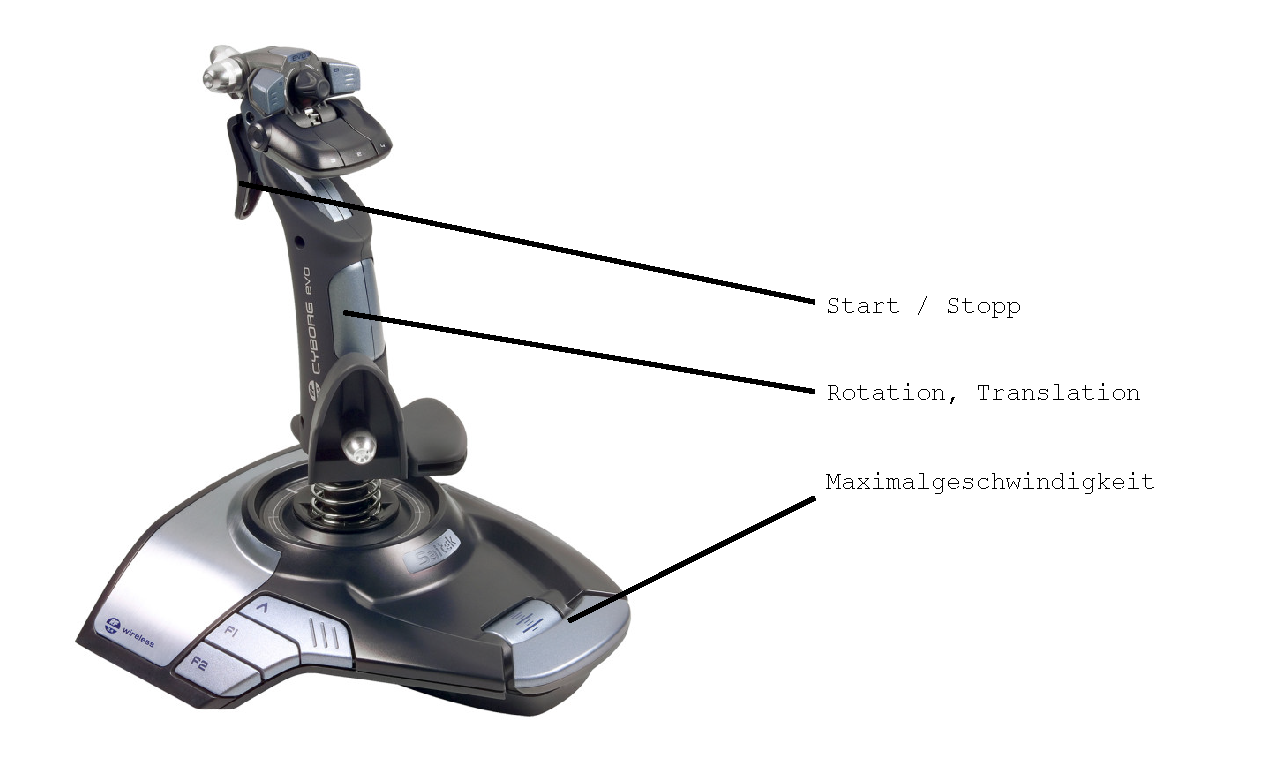
\includegraphics[width=.8\textwidth]{Abbildungen/Joystick}
    \caption{Funktionen des Joysticks}
    \label{fig:Joystick}
\end{figure}

\subsection{Visualisierung}

% !TEX root = Projektstudie.tex
% Fazit

\section{Fazit}
\label{sec:Fazit}

Während zahlreicher Versuchsfahrten stellt sich heraus, dass eine genaue Positionierung nur mit Kenntnis der Radgeschwindigkeiten keine möglich ist.
Kleinste Unebenheiten oder Verschmutzungen resultieren in durchrutschenden oder abhebenden Rädern und somit in starken Fahrbahnabweichungen.
Für den produktiven Betrieb sind daher externe Positionsreferenzen zwingend notwendig.
Weitere Ausführungen dazu folgen im Ausblick (Kapitel~\ref{sec:Ausblick}).

Neben dem Fahrbahnuntergrund erschweren mechanische Probleme ein reibungsloses Fahren des Mecanum-Roboters:

\begin{itemize}
    \item{Die Motoren sind zu schwach dimensioniert und verlieren bei abrupten Manövern Schritte.}
    \item{Das treibende Rad des Riementriebs löst sich nach längerem Gebrauch von der Welle und muss mit gezielten Hammerschlägen wieder an seine Position gebracht werden. Dies hat zur Folge, dass die Mecanum-Räder zu nah am Riementrieb liegen und sich regelmäßig mit den überstehenden Schrauben im Riemen verhaken.}
\end{itemize}

Ein Beheben dieser Probleme setzt eine Neukonstruktion der betrachteten Komponenten voraus. Weitere notwendige Änderungen werden neben Optimierungsansätzen und möglichen folgenden Projekten im Ausblick Kapitel~\ref{sec:Ausblick} beschrieben.

% !TEX root = Projektstudie.tex
% Ausblick

\section{Ausblick}
% - Deckenkamera
% - Hindernissen ausweichen (Dijkstra?)
% - Steuerung übers Netzwerk / W-Lan: Python Flask Server + Raspberry

\end{document}
